\documentclass{article}

\usepackage{hyperref}
\usepackage{graphicx}
\usepackage{amsmath}
\usepackage{float}



\hypersetup{
    colorlinks = true,
    linkcolor = blue,
    anchorcolor = blue
}

\graphicspath{{img/}}





\title{Parallelization of the Game of Life in OpenMPI}

\author{Davide Dal Bianco \\ 2598719}

\begin{document}

\maketitle

\section{Introduction}
The Game of Life has been invented by the mathematician Conway in 1970 where, provided an initial state, the successive states can be computed without any external interaction. Each state consists of a matrix where each cell represents an organism and can be either 0 (dead cell) or 1 (live cell). The successive state can be computed by updating each cell according to the following rules:
\begin{itemize}
    \item If a live cell has less then two adjacent live cells, it will die.
    \item If a live cell has two or three adjacent live cells, it will survive.
    \item If a live cell has more then three adjacent live cells, it will die.
    \item If a dead cell has exactly three adjacent live cells, it will became live.
\end{itemize}
This report aims to summarize the techniques and the algorithm used to parallelize the game of life, starting from the provided sequential version. A basic parallel version is first described and tested and then the program is improved to reach the maximum performance possible. Though the provided sequential program is not the optimal one, the parallel one reflect its main structure in order to provide a fair speedup value.

\section{Parallel algorithm} \label{sec:parallelalgorithm}
The sequential algorithm compute the new state by updating each cell according to the rules of the game. It follows that, for computing a single cell, only the adjacent ones are needed. For this reason, the entire matrix can be distributed among the processes according to a precise partition scheme. The rows partitioning should be the most suitable for this application, which consists in assigning groups of contiguous rows to different processes. This choice is better explained in the paragraph \nameref{sec:blockpartitioning}. \\
Assuming a matrix $N \times M$ and $P$ processes, each process has $\mathcal{O}(N / P)$ rows to compute for each step, thus $\mathcal{O}((M \times N) / P)$ cells. In order to compute a block, a process needs the row that precede and the row that succeed its block, which are owned by another process. For this reason each step introduce a communication of $\mathcal{O}(M)$. The computation comunication ratio is therefore $\mathcal{O}((M \times N) / (P \times M))$, hence the algorithm can perform well only when $P << N$. When the problem size is much greater then the number of rows, the ratio is $\mathcal{O}(N)$ and the algorithm should have a nearly perfect linear speedup.


\subsection{About blocks partitioning} \label{sec:blockpartitioning}
The parallel algorithm uses the rows partitioning scheme to split the matrix among the processes. It differs from blocks partitioning because the blocks width is fixed to the width of the matrix. It can be seen that, when the number of processes is prime, the blocks partitioning coincide with rows partitioning (or columns partitioning), unless more complex solution are used (for example merging adjacent blocks, but this leads to load imbalance problems). \\
Suppose the blocks form a $n \times m$ matrix, hence $P = n \times m$. In both rows and blocks partitioning schemes the computation is the same and is the size of the entire matrix divided by the number of processes, that is $\mathcal{O}((M \times N) / P)$. The amount of communication however might be slightly different. For rows partitioning we already argued that communication is $\mathcal{O}(M)$ and, in particular, it is exactly $2M$ for each iteration. On the other hand, in case of blocks partitioning, the amount of communication needed is $2N/n + 2M/m + 4$, that is, it highly depends on the choice of $P$. For example, if $P = 13$ then $m = 1$ or $n = 1$ and the communication required by rows partitioning is less. If $P = 16$, we can choose $m = 4$ and $n = 4$ and the communication required by blocks partitioning is less. Finally, if we have $P = 17$ we are in the first case again and the communication required by rows partitioning is less. \\
Using blocks partition scheme, each process has to exchange messages with 8 different processes, whilst the rows partitioning scheme requires to communicate with only 2 other processes. \\
We can conclude that rows partitioning performs better since the performance is linear with the number of thread and the communication involve less processes.


\subsection{Rows assignment} \label{sec:rowsassignment}
The rows partitioning scheme should assign the same number of rows to each process, in order to avoid load imbalance problems. However, this is possible only when $N$ is a multiple of $P$. When such condition is not met, we should try to obtain the minimum load imbalance possible, that is, the number of rows per process should be $\lfloor N/P \rfloor$ or $\lceil N/P \rceil$. Given $S = (N~mod~P) \times \lceil N/P \rceil$ and $r = N~mod~P$, the following function $f: Nat \to Nat$ distributes the rows according to the previous criterion:
\[
f(x)=
\begin{cases}
x / \lceil N/P \rceil & if~x < S \\
(x - S) / \lfloor N/P \rfloor + r & if~x \geq S \\
\end{cases}
\]
This function assigns $\lceil N/P \rceil$ rows to the first $N~mod~P$ processes and $\lfloor N/P \rfloor$ to the other ones. $S$ represents the switch point between the two subfunctions and correspond to the number of rows assigned to the first $N~mod~P$ processes. In particular, the function $f$ is a broken line where the slope in the first part is less then the slope in the second part. When $N~mod~P$ is zero, then $S$ is zero and the function is a straight line that assign the same number of rows to each process.

\section{Implementation}
The parallel program has been implemented starting from the sequential one and they share most of the code. The process with rank 0 works as the master node and it also creates the matrix and prints the final result. The sequential program has been modified in this way:
\begin{itemize}
    \item Process with rank 0 creates the matrix and, according to the function defined in the paragraph \nameref{sec:rowsassignment}, send each row to the process that owns it.
    \item Each process receive the rows it owns.
    \item At the beginning of each iteration, each process exchange the boundary rows with the adjacent processes.
    \item At the end of all iterations, each process compute the number of local live cells.
    \item The number of total live cells is collected using \texttt{MPI\_Reduce}.
    \item Process with rank 0 prints the global result.
\end{itemize}
After creating the matrix, process 0 use asynchronous non-blocking sends to spread data among processes. The matrix does not mute, hence buffering the messages is not required. However, before freeing the memory of the matrix it must be ensured that all messages has been received using \texttt{MPI\_Wait}. \\
Due to different startup time and different amount of work (for process 0), some processes might start the iterations before than others ones. In particular, some processes could be start the iterations and be waiting for the boundary rows, while the sending processes might still be in the startup phase. This behaviour is clearly unwanted and it can be avoided using \texttt{MPI\_Barrier} before starting the iterations. This synchronization point allows to start executing the iterations at nearly the same time and avoid distortion in performance measurement. \\
During each iteration processes exchange the boundary rows. A synchronous send is highly unwanted for two reasons: useless synchronization points kill performance and, for this particular communication pattern, it might be possible to reach a deadlock (problem similar to dining philosophers). On the other hand, using non-blocking sends it is not possible to update the matrix until the message has been received. It follows that a process must wait until a message is delivered and this kills the performance again. Asynchonous blocking communication is the best trade off: a small overhead is introduced for copying the message, but the state can be updated even if the messages has not been received. In order to use \texttt{MPI\_Bsend}, MPI require the user to explicitly attach the buffer. The space needed to send a single message with \texttt{MPI\_Bsend} can be obtained using \texttt{MPI\_Pack\_size} and summing the constant \texttt{MPI\_BSEND\_OVERHEAD}, hence multiplying by 4 a lower bound for the buffer size can be calculated (since we use asynchronous communication a process might start the next iteration while the other one has not yet received the data in the current iteration). Note that the order of the two receive must be inverted with respect to the two send to work properly in case there is only one process. However, after implementing the \texttt{MPI\_Bsend}, many executions of the program ended with a buffer overflow exception. The reason can be found in the MPI implementation: though no more of four sends can be pending, there is a delay between when the message is received and when the buffer is freed. It follows that the buffering must be implemented externally with \texttt{MPI\_Isend}. \\
MPI communication tags are not used in the application because the communication scheme is quite easy.


\section{Performance measurement}
The parallel program should have a nearly linear speedup, as we already said in the section \nameref{sec:parallelalgorithm}. In order to measure the performance gain, the running time is measured using \texttt{MPI\_Wtime}, which returns the elapsed time on the calling processor. Once measured the local running times for each processor, we can take the maximum of them as the global running time. Choosing the maximum instead of the average provide a stricter speedup value and penalize load imbalances. However, different executions leads to much different running times. In fact, the execution time of a program is always delayed by a random value, which is even bigger in case of many different systems interconnected. In order to mitigate the effect of random delays, we will run each program four times and we will consider the average running time. \\
The speedup has been measured for three problem sizes:
\begin{itemize}
    \item Size 1: 1000 $\times$ 1000 - 50000 iterations
    \item Size 2: 5000 $\times$ 5000 - 2000 iterations
    \item Size 3: 7500 $\times$ 7500 - 1000 iterations
\end{itemize}
When comparing problem sizes, we compare only the dimensions of the matrix, since the number of iterations and the running time depends linearly. \\
After the first performance measurement a superlinear speedup has been detected. This was not suppose to happen and after further investigation the reason has been found in the copy of the boundary cells. The parallel program first copies the right-left borders and then sends the top-bottom rows (included ghost cells). On the other hand, the sequential program copies the four corner cells separately and this introduce a noticeable overhead. Computer architectures are designed to provide the fastest memory access when reading sequentially. Accessing the memory randomly, like accessing the four corners, has a big impact on performance. For this reason, in order to respect the same structure of the parallel program and provide a fair speedup, \emph{the sequential program has been modified and the four corner cells are now copied together with the top-bottom rows}. \\
\begin{figure}
\centering
\frame{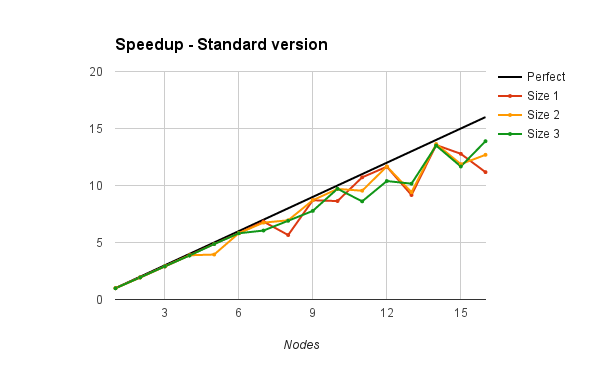
\includegraphics[width=0.8\textwidth]{speedup_standard.png}}
\caption{Speedup - Standard version}
\label{fig:speedupstandard}
\end{figure}
The measured speedup is shown in \autoref{fig:speedupstandard}, or better in \autoref{tab:standardtimes}. After a quick analysis it can be seen that the speedup is neither smooth and close to the perfect linear speedup. In order to understand the reasons of this slow down, the program has been modified to keep track of the execution times of all phases. Since the instructions for monitoring each phase introduce some overhead, they are enabled by the preprocessor only when the word \texttt{DEBUG} is defined. The results are summed up in \autoref{tab:timeperphasecomparison}. We can conclude that the performance loss is caused by the waiting time during the receive phase. Furthermore, the other phases are not communication bounded (the send are nonblocking) and perform computation on data. An attemp to reduce the time of the Receive phase is described in the paragraph \nameref{sec:overlappingcommcomp}.


\begin{table}
\centering
\begin{tabular}{|l|c|c|c|}
\hline
& Size 1 & Size 2 & Size 3 \\
\hline
Boundaries copy & 0.58 (0.09\%) & 0.32 (0.03\%) & 0.39s (0.03\%) \\
\hline
Send & 2.52 (0.39\%) & 0.48 (0.06\%) & 0.41s (0.03\%) \\
\hline
Receive & 22.64 (3.54\%) & 194.81 (23.01\%) & 476.71s (37.95\%) \\
\hline
Update & 469.15 (73.36\%) & 501.71 (59.26\%) & 601.32s (47.88\%) \\
\hline
Matrix copy & 144.65 (22.62\%) & 149.36 (17.64\%) & 177.17s (14.11\%) \\
\hline
\end{tabular}
\caption{Time per phase comparison on 16 nodes} \label{tab:timeperphasecomparison}
\end{table}



\section{Improvements}

\subsection{Memory optimization}
We already discussed the process 0 is the master node, which first create the matrix and then distribute it among all processes. Though this approach is correct and probably the easiest one, it limits the problem size, that is, the matrix must fit in the memory of the master node. \\
We can modify the program in such a way that the matrix must fit in the sum of the memory of all processors. In order to do that, the master node must send the rows immediatly after the creation and free the memory right after the delivery. A synchronous send like \texttt{MPI\_Ssend} is what we need: it blocks until the recipient reads the message and when the call returns we can immediately free the memory. It follows that a node can't send a synchronous message to itself and therefore, instead of using \texttt{MPI\_Ssend}, rows of process 0 are copied manually. Clearly the master node does not have to receive the rows with \texttt{MPI\_Recv} anymore.


\subsection{Overlapping communication and computation} \label{sec:overlappingcommcomp}
In \autoref{tab:timeperphasecomparison} we showed that the receive phase is a bottleneck and the processes spend a noticeable time waiting for the messages. In order to reduce the latencies, we can overlap communication and computation. In fact, the vast majority of the matrix can be computed without the information collected by the receive. Therefore we can exploit the waiting time and compute the inner part of the matrix while messages are in transit. Only when the inner matrix has been computed \texttt{MPI\_Recv} is called to read incoming messages and process the boundary rows. The results are showed in \autoref{fig:speedupoptimized} and listed in \autoref{tab:optimizedtimes}. The performance gain is remarkable and the speedup is now smooth and almost perfect.

\begin{figure}
\centering
\frame{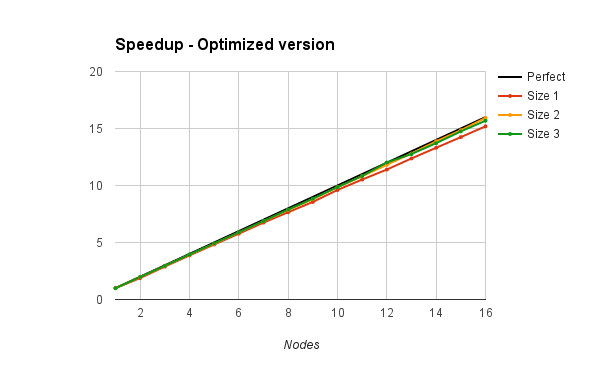
\includegraphics[width=0.8\textwidth]{speedup_optimized.png}}
\caption{Speedup - Optimized version}
\label{fig:speedupoptimized}
\end{figure}


\subsection{Matrix transposition}
The matrix is splitted among processes using the rows partitioning scheme and the communication is $\mathcal{O}(M)$, as described in \nameref{sec:parallelalgorithm}. If the input size of the problem has (much) more columns than rows, a columns partitioning scheme would be slightly better because it requires only $\mathcal{O}(N)$ communication. The easiest way to switch from rows partitioning to columns partitioning is transposing the matrix, since it does not change the result (each cell has the same neighbours). Though, this improvement has not been implemented because the code would be less readable and this application is meant for performance testing. In fact, the problem can be avoided by providing the input dimensions in the opposite order.

\appendix

\section{Execution times}

\begin{table}[H]
\centering
\begin{tabular}{|c|c|c|}
\hline
Size 1 & Size 2 & Size 3 \\
\hline
615.54 & 657.04 & 750.86 \\
\hline
\end{tabular}
\caption{Execution times - Sequential version} \label{tab:sequentialtimes}
\end{table}

\begin{table}[H]
\centering
\begin{tabular}{|l|c|c|c|}
\hline
Nodes & Size 1 & Size 2 & Size 3 \\ \hline
1 & 620.87 (0.99) & 662.75 (0.99) & 762.08 (0.99) \\ \hline
2 & 318.59 (1.93) & 339.00 (1.94) & 388.05 (1.93) \\ \hline
3 & 212.51 (2.90) & 225.60 (2.91) & 258.36 (2.91) \\ \hline
4 & 158.74 (3.88) & 169.09 (3.88) & 194.76 (3.86) \\ \hline
5 & 126.30 (4.87) & 166.34 (3.94) & 154.40 (4.86) \\ \hline
6 & 105.71 (5.82) & 112.81 (5.82) & 129.25 (5.81) \\ \hline
7 & 90.05 (6.84) & 97.29 (6.74) & 124.16 (6.05) \\ \hline
8 & 108.88 (5.65) & 94.46 (6.95) & 108.72 (6.91) \\ \hline
9 & 70.69 (8.71) & 75.32 (8.71) & 96.58 (7.77) \\ \hline
10 & 71.29 (8.63) & 67.65 (9.70) & 77.30 (9.71) \\ \hline
11 & 57.44 (10.72) & 68.75 (9.54) & 87.24 (8.61) \\ \hline
12 & 52.85 (11.65) & 56.23 (11.67) & 72.26 (10.39) \\ \hline
13 & 67.18 (9.16) & 69.70 (9.41) & 73.91 (10.16) \\ \hline
14 & 45.43 (13.55) & 48.10 (13.64) & 55.62 (13.50) \\ \hline
15 & 48.17 (12.78) & 55.26 (11.87) & 64.35 (11.67) \\ \hline
16 & 55.11 (11.17) & 51.70 (12.69) & 54.07 (13.89) \\ \hline
\end{tabular}
\caption{Execution times - Standard version} \label{tab:standardtimes}
\end{table}

\begin{table}[H]
\centering
\begin{tabular}{|l|c|c|c|}
\hline
Nodes & Size 1 & Size 2 & Size 3 \\ \hline
1 & 617.03 (1.00) & 661.51 (0.99) & 754.20 (1.00) \\ \hline
2 & 328.02 (1.88) & 335.01 (1.96) & 380.39 (1.97) \\ \hline
3 & 213.16 (2.89) & 222.63 (2.95) & 253.93 (2.96) \\ \hline
4 & 159.26 (3.87) & 166.86 (3.93) & 190.22 (3.95) \\ \hline
5 & 127.61 (4.82) & 134.19 (4.89) & 152.43 (4.93) \\ \hline
6 & 106.63 (5.77) & 111.58 (5.88) & 127.35 (5.90) \\ \hline
7 & 91.31 (6.74) & 95.63 (6.86) & 109.11 (6.88) \\ \hline
8 & 80.41 (7.66) & 83.56 (7.85) & 95.18 (7.89) \\ \hline
9 & 71.91 (8.56) & 74.53 (8.80) & 84.88 (8.85) \\ \hline
10 & 64.08 (9.61) & 66.63 (9.85) & 76.15 (9.86) \\ \hline
11 & 58.50 (10.52) & 60.68 (10.81) & 69.30 (10.84) \\ \hline
12 & 54.00 (11.40) & 55.53 (11.81) & 62.47 (12.02) \\ \hline
13 & 49.75 (12.37) & 51.23 (12.81) & 58.83 (12.76) \\ \hline
14 & 46.25 (13.31) & 47.26 (13.88) & 54.75 (13.71) \\ \hline
15 & 43.22 (14.24) & 44.19 (14.84) & 50.92 (14.75) \\ \hline
16 & 40.52 (15.19) & 41.17 (15.93) & 47.88 (15.68) \\ \hline
\end{tabular}
\caption{Execution times - Optimized version} \label{tab:optimizedtimes}
\end{table}

\end{document}